\documentclass[aspectratio=169,11pt]{beamer}

% Shared style (ib-tutorials.sty at the repo root).
\makeatletter\def\input@path{{./}{../}}\makeatother
\usepackage{ib-tutorials}

\usepackage[utf8]{inputenc}
\usepackage{amsmath,amssymb}
\usepackage{booktabs}
\usepackage{array}
\newcolumntype{L}[1]{>{\raggedright\arraybackslash}p{#1}}
\usepackage{graphicx}
\graphicspath{{../pictures/2-ib2d/}{pictures/2-ib2d/}}
\usepackage{xcolor}
\usepackage{listings}
\usepackage{tikz}
\usetikzlibrary{arrows.meta,positioning,shapes.geometric,fit,calc}
\usepackage{hyperref}

\newcommand{\sourcecredit}[1]{\vfill\hfill{\tiny\textcolor{DarkGray}{#1}}}
\newcommand{\gui}[1]{\textsf{\textbf{#1}}}

\lstset{
  basicstyle=\ttfamily\scriptsize\color{BlackGray},
  keywordstyle=\color{NavyBlue}\bfseries,
  commentstyle=\color{DarkGray}\itshape,
  stringstyle=\color{OliveGreen},
  showstringspaces=false,
  columns=fullflexible,
  keepspaces=true,
  breaklines=true,
  frame=single,
  framerule=0.4pt,
  rulecolor=\color{LightGray},
  backgroundcolor=\color{LightGray!30},
  xleftmargin=0.25em,
  xrightmargin=0.25em
}
\lstdefinestyle{shell}{morecomment=[l]{\#}}
\lstdefinestyle{input}{morecomment=[l]{\%}}
\lstdefinestyle{plain}{}
\lstdefinestyle{py}{language=Python}
\lstdefinestyle{m}{language=Matlab}
\lstdefinestyle{tiny}{basicstyle=\ttfamily\tiny\color{BlackGray}}
\lstdefinestyle{pytiny}{language=Python,basicstyle=\ttfamily\tiny\color{BlackGray}}

\title[IB2d: moving boundaries, your own example]{Moving boundaries, and making your own example}
\subtitle{The \code{update\_*} functions that move target points, change springs and bend beams in time; the moving band and the sawtooth pump, run in Python; the two styles of prescribing motion; a geometry of your own from a sketch to a running folder}
\author[Miller]{Laura A. Miller}
\institute[UArizona]{Department of Mathematics, University of Arizona}
\date{Using IB Software \textbullet\ Part II \textbullet\ Chapter 4c}

\begin{document}

% ---------------------------------------------------------------- title
\begin{frame}[plain]
\maketutorialtitlepanel{%
\begin{tikzpicture}[scale=0.95]
  \draw[DarkGray,thick] (0,0) rectangle (4,4);
  \draw[BlackGray,very thick] (0.4,2.9) -- (0.8,3.5) -- (1.2,2.9) -- (1.6,3.5) -- (2.0,2.9) -- (2.4,3.5) -- (2.8,2.9) -- (3.2,3.5) -- (3.6,2.9);
  \draw[RubineRed,very thick] (0.4,1.1) -- (0.8,1.7) -- (1.2,1.1) -- (1.6,1.7) -- (2.0,1.1) -- (2.4,1.7) -- (2.8,1.1) -- (3.2,1.7) -- (3.6,1.1);
  \draw[-{Latex[length=2mm]},RubineRed,thick] (2.0,0.5) -- (2.0,0.95);
  \draw[-{Latex[length=2mm]},RubineRed,thick] (2.0,2.35) -- (2.0,1.9);
  \node[font=\tiny,NavyBlue] at (2,0.2) {\code{update\_Target\_Point\_Positions}};
\end{tikzpicture}}
\end{frame}

% ---------------------------------------------------------------- goals, sources
\begin{frame}{What you will be able to do after this chapter}
\label{fr:goals}
\footnotesize
\begin{itemize}
  \item Name the four ways a boundary moves in IB2d (target points, springs, beams, muscles), the \code{input2d} flag and the function file behind each, and what the driver passes to that function.
  \item Write an \code{update\_Target\_Point\_Positions} function: the moving band (every point dragged along a path), the sawtooth pump (one row of a channel driven in time) and the pulsing heart (every point blended between two shapes), all three in Python.
  \item Choose between the two ways of prescribing a motion (increment the targets every step, or set them from the original positions) and know why the second one does not drift.
  \item Change spring resting lengths and beam curvatures in time with the same mechanism (the impedance pump and the swimmer of chapter 4b).
  \item Build an example of your own from a sketch: domain, grid, points at $\Delta x/2$, indices, the files, the flags, a short first run, the checks.
\end{itemize}
\begin{punchbox}
\small Three examples were ported to Python and run in October 2026 (\code{examples/IB2d/Moving\_Rubberband}, \code{Sawtooth}, \code{Pulsing\_Heart} in the repository); the ports reproduce the MATLAB geometry files to round-off ($2 \cdot 10^{-15}$). The MATLAB sawtooth is a $1024 \times 256$ run of hours and did not survive on any laptop grid tried (slide \ref{fr:sawrun}): it is the chapter's cautionary case; the pulsing heart is its working pump.
\end{punchbox}
\end{frame}

\begin{frame}{Where this chapter comes from}
\label{fr:sources}
\footnotesize
\begin{itemize}
  \item \al{``Changing target positions'' (Lecture 3 of the 2022 UA tutorials, 20 slides; its IB2d half, slides 3--13):} the four ways to move a boundary, the sawtooth example line by line (\code{give\_Me\_Sawtooth\_Geometry}, what it prints, \code{update\_Target\_Point\_Positions}, \code{N\_top}), and the IBAMR half that is chapter 9a.
  \item \al{Lectures 11 and 12 (2021--23):} the same sawtooth block, the homework, and (Lecture 12) the stability material that is chapter 4d; the 2024 practical's slide 29 repeats the four-way list.
  \item \al{``IB2d and IBAMR associated files'' (Lecture 2, 2022), slides 20--24 and 32--38:} creating geometries ($\Delta s = \Delta x/2$, the origin, fitting the box), the rubber-band generator in both flavours, the MATLAB checkers, the project ideas.
  \item \al{The course's ``4-ib2d-MakeYourOwnExample'' folder (two beams driven by target points) and its homework} (``Your own rubber band'', Lectures 3 and 9; option 2 of Lecture 11's homework 4).
  \item The IB2d examples \code{Example\_Moving\_Rubberband}, \code{Example\_Sawtooth}, \code{Example\_Pulsing\_Heart} (all three ported here), \code{Tracers\_In\_Impedance\_Pump} (Python) and the swimmer (chapter 4b).
\end{itemize}
What is new here: the three Python ports and their runs, the two prescription styles, the sawtooth's failure on laptop grids, the checklist for a new example, and three things to fix in the course's own template.
\end{frame}

% ---------------------------------------------------------------- the mechanism
\begin{frame}{Four ways to move a boundary, one mechanism}
\label{fr:four}
\scriptsize
\begin{tabular}{@{}L{0.17\textwidth}L{0.22\textwidth}L{0.33\textwidth}L{0.20\textwidth}@{}}
\toprule
Move it by & \code{input2d} & the function the driver calls every step & the table it edits \\
\midrule
target points that travel & \code{target\_pts = 1}, \code{update\_target = 1} & \code{update\_Target\_Point\_Positions(dt, current\_time, targets)} & index, $x$, $y$, $k_t$ \\
springs whose $k$ or $L$ change & \code{springs = 1}, \code{update\_springs = 1} & \code{update\_Springs(dt, current\_time, xLag, yLag, springs)} & $i$, $j$, $k$, $L$, $\alpha$ \\
beams whose rest curvature changes & \code{beams = 1}, \code{update\_beams = 1} (or the \code{nonInv} pair) & \code{update\_Beams(dt, current\_time, beams)}, \code{update\_nonInv\_Beams(\ldots)} & $i$, $j$, $k$, $k_b$, $C$ (or $C_x$, $C_y$) \\
damped springs & \code{damped\_springs = 1}, \code{update\_damp\_springs = 1} & \code{update\_Damped\_Springs(dt, current\_time, d\_springs)} & $i$, $j$, $k$, $L$, $b$ \\
muscles & \code{FV\_LT\_muscle = 1} & an activation function you write (chapter 4e) & \\
\bottomrule
\end{tabular}
\end{frame}

\begin{frame}{How the driver uses the update functions}
\label{fr:four2}
\small
\begin{itemize}
  \item The function lives in the example folder, \code{.m} for MATLAB, \code{.py} for Python (the Python driver does \code{from update\_Springs import update\_Springs} inside the step loop). The driver calls it once per step, after the half-step move of the points and before the forces are computed, and \al{replaces the table with what the function returns}.
  \item The structure's own positions are never set by these functions: a target moves, and the point follows it through the target force $k_t (\mathbf{X}^{\mathrm{target}} - \mathbf{X})$ (chapter 4a); a resting length changes, and the spring pulls. That is why the motion is ``approximately prescribed'' and why the stiffness matters (slide \ref{fr:sawrun}).
  \item Lecture 3's list: ``target points to provide a preferred motion; springs whose stiffness or resting lengths change in time; beams whose resting curvature changes in time; muscle models / muscle springs''; Lectures 11 and 12 add ``This is typically done by making an \code{update\_XXX.m} or \code{.py} file.''
\end{itemize}
\end{frame}

\begin{frame}{The target table}
\label{fr:table}
\small
\begin{columns}[T]
\column{0.5\textwidth}
\begin{tabular}{@{}L{0.14\textwidth}L{0.76\textwidth}@{}}
\toprule
column & MATLAB (1-based) / Python (0-based) \\
\midrule
1 / 0 & the point's index in the \code{.vertex} order \\
2 / 1 & the target's $x$ \\
3 / 2 & the target's $y$ \\
4 / 3 & the stiffness $k_t$ from the \code{.target} file \\
\bottomrule
\end{tabular}

\vspace{2mm}
\begin{itemize}
  \item Built by the driver from the \code{.target} file and the initial \code{.vertex} positions, in the order of the \code{.target} file; the table's row $r$ is the target of point \code{targets(r, 1)}.
  \item The examples write a \code{.target} line for every point in order, so row $r$ is point $r$; a file that lists a subset of points, or in another order, breaks that habit, and the index column is there for it.
\end{itemize}
\column{0.48\textwidth}
\begin{itemize}
  \item Change columns 2--3 (MATLAB) or 1--2 (Python) and return the table: the targets have moved. Change column 4/3 and the tether stiffens or loosens (a way to release a structure at a given time).
  \item \code{current\_time} is the time at the start of the step; \code{dt} the step. A motion written as a function of \code{current\_time} is exact; one written as an increment per step accumulates (slide \ref{fr:styles}).
  \item Lecture 3: ``you need to loop through all vertices and determine which to move (1--3276) and which to not move (3277--6552)'', which is why the generator prints the counts (slide \ref{fr:sawgen}).
\end{itemize}
\end{columns}
\end{frame}

% ---------------------------------------------------------------- example 1: the moving band
\begin{frame}[fragile]{Example 1: the moving band (\code{Example\_Moving\_Rubberband}, in Python)}
\label{fr:band}
\begin{columns}[T]
\column{0.5\textwidth}
\begin{lstlisting}[style=py]
def update_Target_Point_Positions(dt, current_time, targets):
    period = 0.05            # time of one right-or-left leg
    L = 0.5                  # distance travelled in each direction
    s = L / (period / 2)     # speed
    t = current_time % period
    targets[:, 2] += (s / 2) * dt        # up, always
    if t < period / 2:
        targets[:, 1] += s * dt          # right
    else:
        targets[:, 1] -= s * dt          # left
    return targets
\end{lstlisting}
\small
The MATLAB original loops over the rows and does the same (\code{targets(IDs(i),3) = yPts(IDs(i)) + (s/2)*dt} and the $x$ branch); the Python port uses the table's columns at once.
\column{0.48\textwidth}
\small
\begin{itemize}
  \item A circle of 64 target points ($k_t = 10^7$) centred at (0.25, 0.25), in a viscous fluid ($\mu = 10$, $\rho = 1$), $32^2$, $\Delta t = 10^{-4}$, $T = 0.05$, a dump every 5 steps.
  \item Every step the targets move right (first half of the period) or left (second half) at speed 20 and up at speed 10: a zig-zag of two legs of 0.5.
  \item Files: \code{Rubberband.py} (the generator: \code{.vertex} and \code{.target}, 0-based), \code{update\_Target\_Point\_Positions.py}, \code{input2d} with \code{target\_pts = 1} and \code{update\_target = 1}, \code{main2d.py}.
  \item 2.9 s for 500 steps; 100 dumps.
\end{itemize}
\end{columns}
\end{frame}

\begin{frame}{The moving band: what happens}
\label{fr:bandpic}
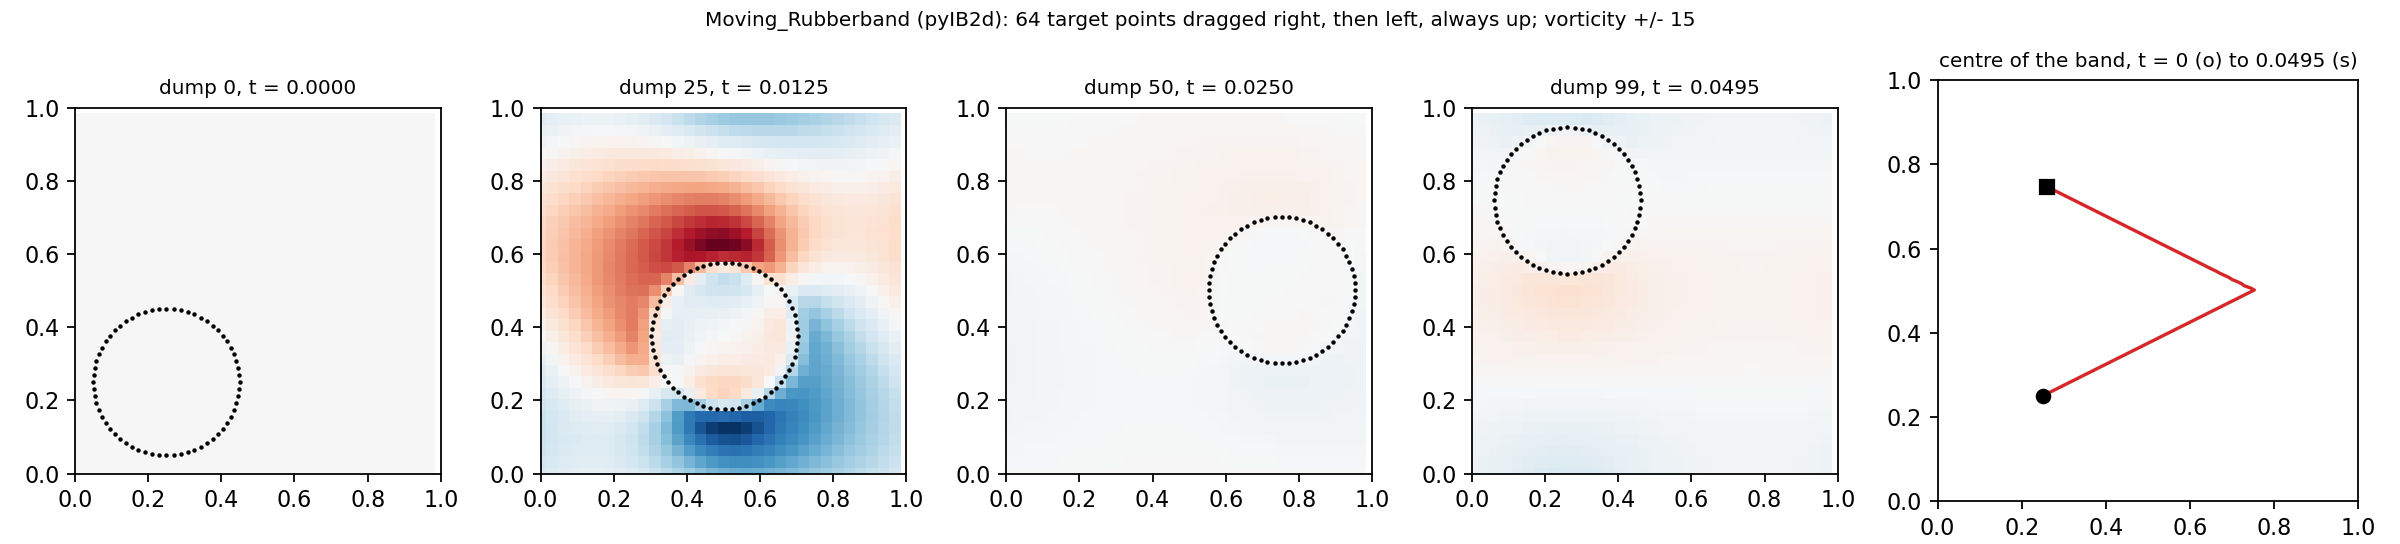
\includegraphics[width=\textwidth]{ch4c-moving-band.png}
\small
\begin{itemize}
  \item The band's centre goes from (0.25, 0.25) to (0.75, 0.50) at $t = 0.025$ and back to (0.26, 0.75) at the end: the two legs of the zig-zag (right panel). The points keep up with their targets because $k_t$ is large and the fluid is viscous; the vorticity ($\pm 15$ in the frames shown) is the wake of a cylinder dragged through a viscous fluid; the reversal of the target velocity at $t = 0.025$ produces a spike of 840 one dump later that decays within a few dumps: an instantaneous change of a prescribed velocity is a jolt, and a smooth reversal (slide \ref{fr:phases}) would avoid it.
  \item Nothing in the \code{.vertex} file knows about the motion: the same files with \code{update\_target = 0} give a band that sits still. The motion is in the function, and the fluid responds.
\end{itemize}
\end{frame}

\begin{frame}[fragile]{Two ways to prescribe a motion}
\label{fr:styles}
\begin{columns}[T]
\column{0.5\textwidth}
\footnotesize
\al{Increment every step} (the moving band):
\begin{lstlisting}[style=py]
targets[:, 1] += s * dt
\end{lstlisting}
\begin{itemize}
  \item Short to write; the motion is whatever the increments add up to.
  \item The position after $n$ steps is $n\, s\, \Delta t$ in floating point, and the leg changes direction when \code{t < period/2} flips, which depends on how \code{current\_time} is accumulated; change $\Delta t$ and the turning point moves by up to one step. Over many periods the table drifts from where the formula says.
\end{itemize}
\column{0.48\textwidth}
\footnotesize
\al{Set from the original positions} (the sawtooth):
\begin{lstlisting}[style=py]
shift = (a / 2) * sin(2 * pi * freq * current_time)
for i in range(N_top):
    targets[i, 2] = y0[i] - shift
\end{lstlisting}
\begin{itemize}
  \item The targets are a function of time and of the original geometry (\code{y0}, read once from the \code{.vertex} file): no drift, the same motion at every $\Delta t$, and a restart from any time is exact.
  \item Lecture 3: ``this code is written such that the new positions are calculated using the original positions. You could also modify based on the position from the previous time step.'' Prefer the first.
\end{itemize}
\end{columns}
\begin{punchbox}
\small Both styles are fine for a demonstration; for a study (a resolution or time-step sweep, chapter 4d) use the second, so that the prescribed motion is identical across the runs you compare.
\end{punchbox}
\end{frame}

% ---------------------------------------------------------------- example 2: the sawtooth
\begin{frame}[fragile]{Example 2: the sawtooth pump: the geometry}
\label{fr:sawgen}
\begin{columns}[T]
\column{0.5\textwidth}
\begin{lstlisting}[language=Matlab,basicstyle=\ttfamily\tiny\color{BlackGray}]
Lx = 12;  Ly = 3.0;             % the box
Nx = 1024;  Ny = 256;           % chosen so that dx = dy
ds = Lx/(2.1*Nx);               % a little under dx/2
d = 0.63;  w = 0.63;            % tooth height and width
G = 0.325;                      % vertical gap between the rows
[xLag, yLag] = give_Me_Lagrangian_Geometry(ds,d,w,G);
xLag = xLag + ( Lx/2 - xLag(end/4) );  % centre in x
yLag = yLag + ( Ly/2 );                % centre in y
fprintf('G = %d (vertical gap btwn top and bottom)\n',G);
fprintf('N_Top = %d (# of points on top of sawtooth)\n', length(xLag)/2);
k_Target = 1e11;
print_Lagrangian_Target_Pts(xLag,k_Target,struct_name);
\end{lstlisting}
\footnotesize \code{give\_Me\_Sawtooth\_Geometry.m}, abridged. One tooth is a vertical rise of $d$ followed by a diagonal down to $(w, 0)$; 12 teeth make the top row at $+G/2$, their mirror image the bottom row at $-G/2$.
\column{0.48\textwidth}
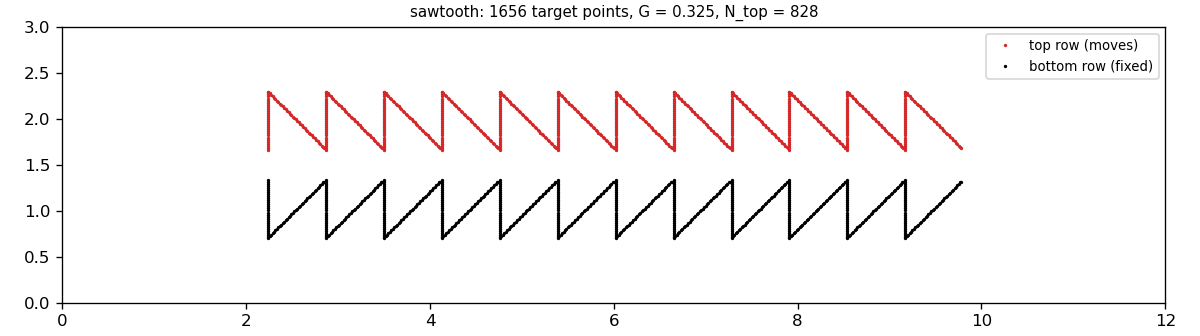
\includegraphics[width=0.95\textwidth]{ch4c-sawtooth-geometry.png}
\scriptsize The generator's own figure at $256 \times 64$: the top row (red) is the one that moves.
\end{columns}
\end{frame}

\begin{frame}{The sawtooth's numbers}
\label{fr:sawgen2}
\small
\begin{itemize}
  \item 6552 target points at $1024 \times 256$ ($\Delta s = 0.48\,\Delta x$), 1656 at $256 \times 64$ (the Python port's default): \al{the top row first, then the bottom row}, which is the whole trick of the update function.
  \item The generator prints \code{G} and \code{N\_Top} because the update function needs them: ``if you change the geometry or the resolution, you need to update the function \ldots\ manually'' (Lecture 3). The Python port reads \code{N\_top} from the file instead (next slide).
  \item $\mu = 2.234$, $\rho = 1000$, $\Delta t = 2.5 \cdot 10^{-5}$, $T = 10$, a dump every 400 steps: an SI-flavoured set-up (water, a 12 m channel) that is dimensionless in effect.
\end{itemize}
\end{frame}

\begin{frame}[fragile]{The sawtooth pump: the update function}
\label{fr:sawupd}
\begin{columns}[T]
\column{0.46\textwidth}
\begin{lstlisting}[style=m]
function targets = update_Target_Point_Positions(dt,current_time,targets)
freq = 2;        % pumping frequency
a = 0.337;       % total vertical distance the pump travels
N_top = 3276;    % # of points along top
yPTS = read_In_yPT_Positions('sawtooth.vertex');
targets(1:N_top,3) = yPTS(1:N_top) ...
    - (a/2)*sin( 2*pi*freq*current_time );
\end{lstlisting}
\small The MATLAB function, abridged (\code{read\_In\_yPT\_Positions} is its own helper).
\column{0.52\textwidth}
\begin{lstlisting}[style=py]
# Python port: N_top from the file, the originals read once
def update_Target_Point_Positions(dt, current_time, targets):
    if _y0 is None:
        _original_positions()       # reads sawtooth.vertex; N_top = n // 2
    shift = (a / 2) * math.sin(
        2 * math.pi * freq * current_time)
    for i in range(_N_top):
        targets[i, 2] = _y0[i] - shift
    return targets
\end{lstlisting}
\small The Python port (\code{examples/IB2d/Sawtooth/}\allowbreak\code{update\_Target\_Point\_Positions.py}).
\end{columns}
\end{frame}

\begin{frame}{The update function: what it does, and the trap in it}
\label{fr:sawupd2}
\small
\begin{itemize}
  \item The top row moves down and up as a sine of amplitude $a/2 = 0.1685$ at 2 cycles per unit time; the bottom row keeps its targets. The rows' tips are $G = 0.325$ apart, so the stroke ($a/2 \approx G/2$) brings the top row down to the channel's centreline and halves the gap (Lecture 3: ``the gap is 0.325, and the pump will move down by a/2. Make sure the top and bottom don't collide''). The file's commented-out lines (\code{occ = 0.95}) belong to a version in which the bottom row rises too, for 95\,\% occlusion.
  \item The MATLAB version re-reads the \code{.vertex} file at every step (``\code{yPTS = read\_In\_yPT\_Positions}''): 6552 lines, 400\,000 times over the run. The port reads once.
  \item To move the bottom row too: ``\code{targets(N\_top+1:2*N\_top,3) = yPTS(N\_top+1:2*N\_top) + movement\_function}'' (Lecture 3); in antiphase, the channel squeezes symmetrically.
  \item \code{N\_top} is the hard-coded number that bites when the grid changes: 3276 at $1024 \times 256$, 828 at $256 \times 64$. A function that counts the file's points, or a generator that writes the count into a small file the function reads, removes the trap.
\end{itemize}
\end{frame}

\begin{frame}{Running the sawtooth on a quarter of the grid: the stiffness lesson}
\label{fr:sawrun}
\scriptsize\setlength{\itemsep}{1pt}
\begin{itemize}
  \item The MATLAB example is a $1024 \times 256$ grid for 400\,000 steps: hours. The Python port takes the grid as an argument; at $256 \times 64$ (1656 points) a step takes 0.01--0.04 s on a laptop, so one pumping cycle ($T = 0.5$, 20\,000 steps) would be a run of 4--14 minutes. None of the runs reached it.
  \item \al{As shipped it blows up}: with $k_t = 10^{11}$ and $\Delta t = 2.5 \cdot 10^{-5}$ the coarse run produces \code{NaN} positions at $t = 0.02$ (an \code{IndexError} from the delta-function indices is how Python reports it). The same $\Delta t$ with $k_t = 10^9$ fails at $t = 0.03$, with $10^8$ at $t = 0.065$ (and at $t = 0.068$ with $\Delta t = 10^{-5}$: not a time-step limit); $10^7$ survives the longest, past $t = 0.12$, with the top row near the centreline; shorter strokes ($a = 0.25$, $0.30$) with $10^7$ fail at $t = 0.15$ and $0.13$ (all times are those of the last dump before the failure).
  \item \al{Softer is not the answer either}: with $k_t = 10^7$ the worst point of the moving row is 0.09, two cells, from its target at $t = 0.1$ (the tooth tips are dragged sideways; the row's mean lag is a fifth of a cell), and the bottom row's tips have begun to shed points (next slide): the tether no longer holds the wall against the flow it drives.
  \item \al{Nor is a shorter channel at the original resolution}: four teeth in a $4 \times 2$ box on $384 \times 192$ ($\Delta x = 0.0104$, the original's $0.0117$) with $k_t = 10^{11}$ ran past $t = 0.21$ and failed on the up-stroke; with $10^{10}$ at $t = 0.02$.
  \item The lesson: a pump whose walls come within a few cells of each other is the hardest case for a tethered boundary; this one was tuned for its grid, its stiffness and its step together, and no single knob transplants it to a laptop. Chapter 4d measures what each knob does on the rubber band; the working low-resolution pump of this chapter is the pulsing heart (slide \ref{fr:heart}).
\end{itemize}
\begin{punchbox}
\small Lecture 12's stability slides (``the time step necessary for stability is inversely proportional to the force applied to the fluid; the forcing term is typically what causes the instability, not the CFL condition'') are chapter 4d, which measures exactly this on the rubber band and on this pump.
\end{punchbox}
\end{frame}

\begin{frame}{The sawtooth pump: what it does}
\label{fr:sawpic}
\begin{center}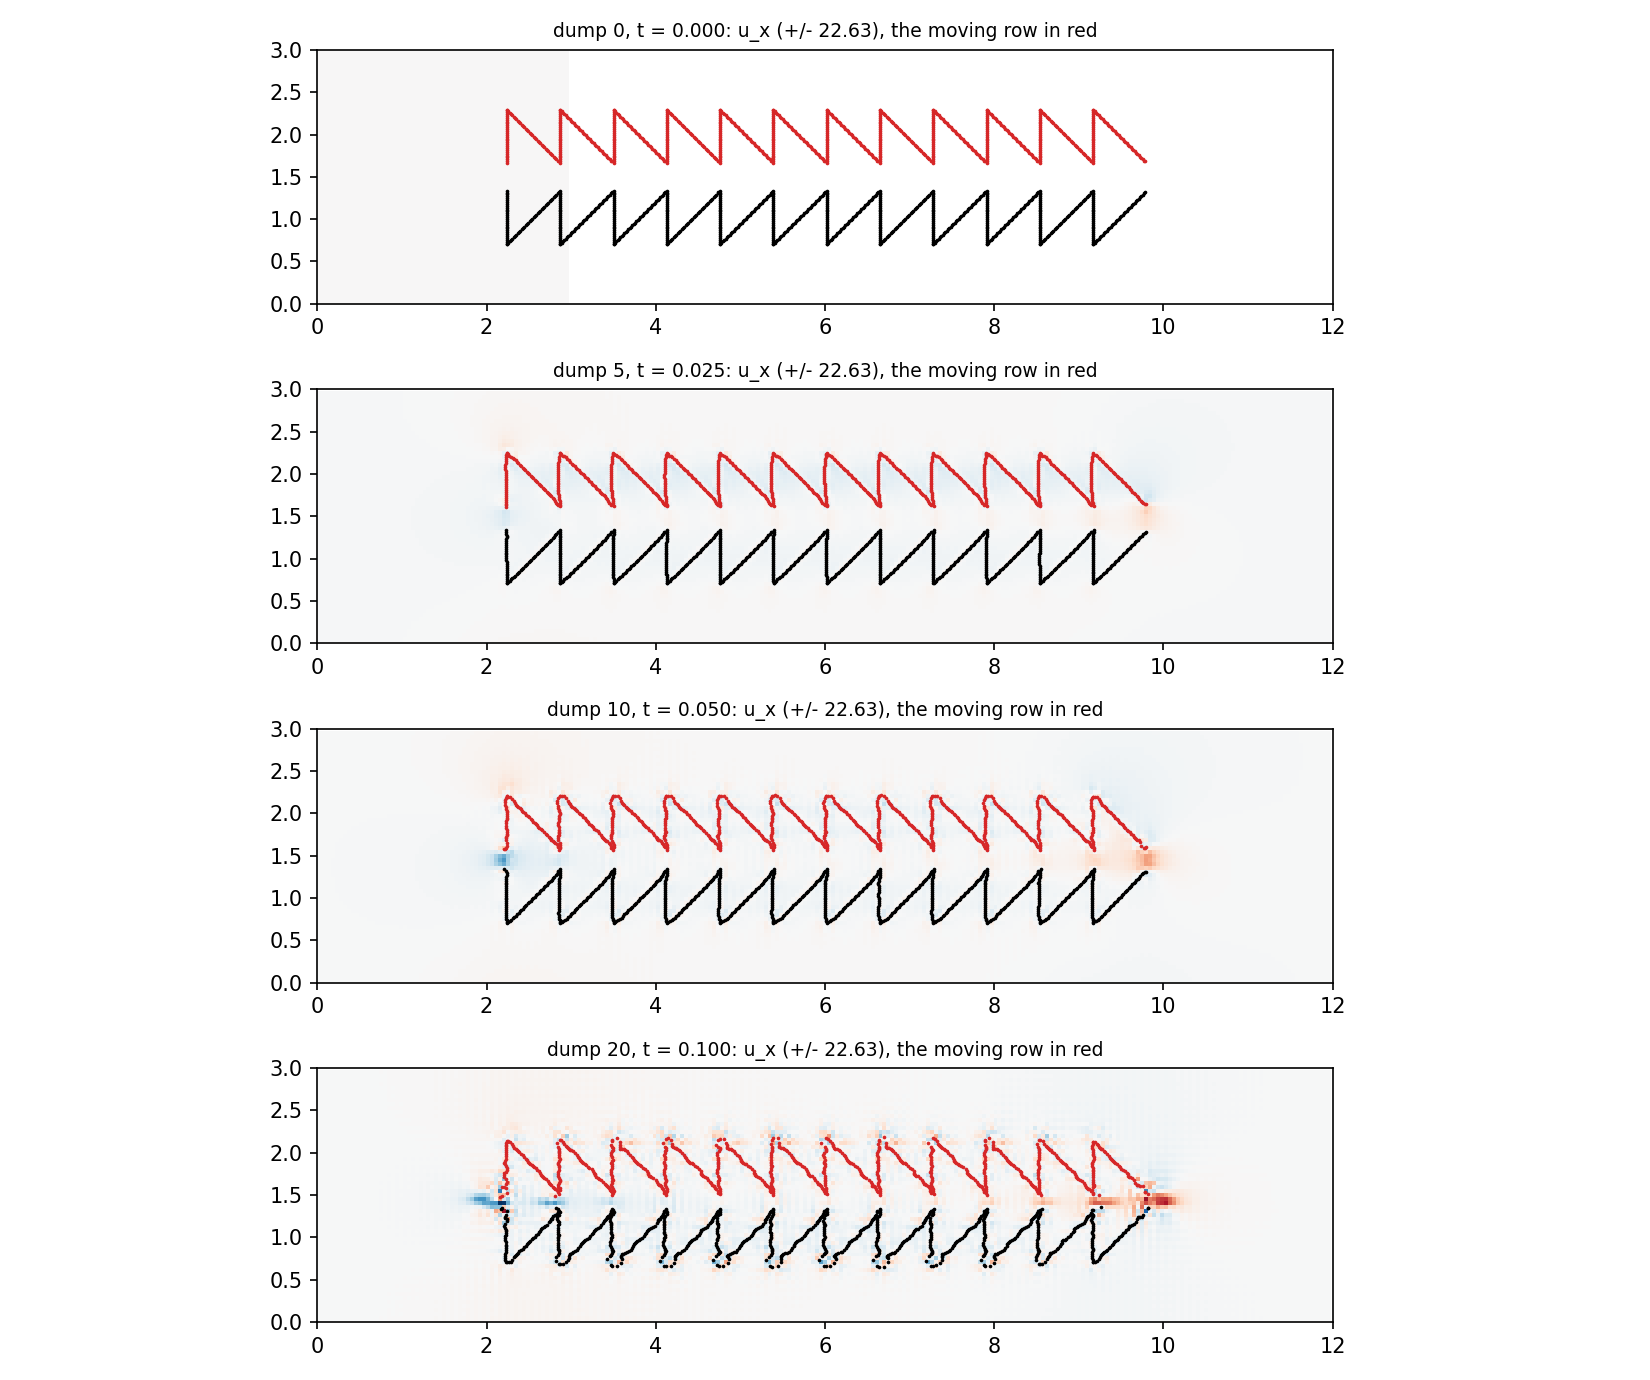
\includegraphics[height=0.62\textheight]{ch4c-sawtooth-frames.png}\end{center}
\footnotesize $u_x$ at four times of the first tenth of a second ($256 \times 64$, $k_t = 10^7$), the moving row in red; the colour scale is the largest $|u_x|$ of the four frames. The down-stroke pushes fluid out of both ends of the channel; by $t = 0.1$ the lower row's tips have begun to shed points (the tether is too soft to hold them), and the run fails at $t = 0.12$.
\end{frame}

\begin{frame}{The sawtooth pump: the flow it drives}
\label{fr:sawflux}
\begin{columns}[T]
\column{0.42\textwidth}
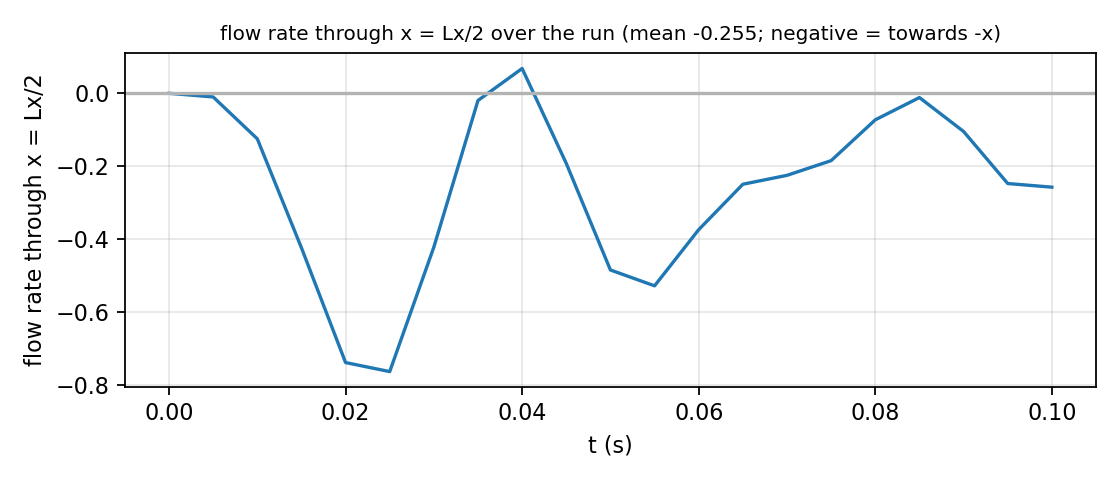
\includegraphics[width=\textwidth]{ch4c-sawtooth-flux.png}
\column{0.56\textwidth}
\footnotesize
\begin{itemize}
  \item The flow rate through the channel's middle, $\int u_x\, dy$ at $x = L_x/2$, over the tenth of a second the run lasted: towards $-x$ after the first few dumps (one small positive excursion at $t = 0.04$), $-0.76$ at most, $-0.26$ on average. A full cycle, and so the net pumping, was not reached (previous slides). The MATLAB example's \code{Sawtooth\_Data\_Analysis.m} does the measurement differently: it averages the speed over a window at each end of the channel for the first three of the run's twenty cycles.
  \item The teeth make the two half-strokes unequal, which is how a symmetric sine of the wall pumps in one direction (Lecture 3's one-line description: ``the top of the channel moves up and down to drive flow''). Chapter 4e has the pumps that do it with resting lengths and with muscles; the next slides have the one that runs on a laptop.
\end{itemize}
\end{columns}
\end{frame}

% ---------------------------------------------------------------- springs and beams in time
\begin{frame}[fragile]{The same mechanism for springs and beams}
\label{fr:springs}
\begin{columns}[T]
\column{0.5\textwidth}
\small
\al{Resting lengths} (\code{Tracers\_In\_Impedance\_Pump}, Python; chapter 4b):\footnotesize
\begin{lstlisting}[style=pytiny]
def update_Springs(dt, current_time, xLag, yLag, springs):
    # springs: columns 0-1 the two points, 2 k, 3 the resting length, 4 alpha
    ...                                  # choose the rows of one section of the tube
    springs[rows, 3] = L0 * (1 - amp * f(current_time))   # pinch: shorter rest length
    return springs
\end{lstlisting}
\begin{itemize}
  \item The pinch is a shorter resting length for the springs across one section of the tube at the right phase; the walls pull in, the fluid is squeezed; tracers show the net transport (chapter 4b's picture).
  \item The heart tubes of \code{Example\_HeartTube} do the same with a travelling wave (``dynamic suction pumping'' and ``peristaltic waves of contraction'' in the example list) and, in the muscle versions, with an activation function instead (chapter 4e).
\end{itemize}
\end{columns}
\end{frame}

\begin{frame}[fragile]{The same mechanism for beams}
\label{fr:beams}
\begin{columns}[T]
\column{0.5\textwidth}
\small
\al{Rest curvature} (the swimmer, MATLAB; chapter 4b):
\begin{lstlisting}[style=tiny]
function beams_info = update_nonInv_Beams(dt,current_time,beams_info)
% beams_info: col 1-3 the points, col 4 k_b, col 5 Cx, col 6 Cy
t = rem(current_time, period);      % time within the stroke
...                                  % blend the two stored phases at t
beams_info(:,5) = Cx_t;  beams_info(:,6) = Cy_t;
\end{lstlisting}
\column{0.48\textwidth}
\small
\begin{itemize}
  \item The preferred shape is stored as two phases (\code{swimmer.phases}); the function blends them at the current time and writes the second differences into the curvature columns. The beam bends towards the new shape, the fluid pushes back, and the swimmer swims.
  \item \code{update\_Beams} does the same with the scalar $C$ of the torsional beams; \code{update\_Damped\_Springs} with $k$, $L$, $b$.
  \item Every table keeps its first columns (the indices) untouched: the connectivity is fixed for the run. A structure that changes topology (a valve that detaches) is not an \code{update\_*} job.
\end{itemize}
\end{columns}
\end{frame}

\begin{frame}{Interpolating between phases (the pulsing heart)}
\label{fr:phases}
\small
\begin{itemize}
  \item \code{Example\_Pulsing\_Heart}: a cartoon heart whose target points interpolate between two stored shapes (``interpolates between two phases'', the example list), with a $32 \times 32$ and a $512 \times 512$ version; the swimmer stores two shapes the same way (their curvatures are computed in the function).
  \item The pattern: the generator writes the geometry at phase A as the \code{.vertex} file and the geometry at phase B as a second file (or a second column set); the update function reads both once, and sets the targets to $(1 - \theta(t))\,\mathbf{X}_A + \theta(t)\,\mathbf{X}_B$ with $\theta$ a smooth 0-to-1-to-0 function of the time within the period (the swimmer's quadratic--cubic--quadratic blend is one; $\tfrac12(1 - \cos 2\pi t/P)$ is another).
  \item It is the second style of slide \ref{fr:styles} with the geometry drawn twice instead of written as a formula: the way to prescribe a motion traced from images (a bell, a heart, a fin), with as many phases as the images give.
  \item The same two-state interpolation drives IBAMR's target points in chapter 9a; chapter 20's IBFE active stress prescribes a travelling wave instead of two shapes. What changes is only where the function lives.
\end{itemize}
\end{frame}

\begin{frame}[fragile]{Example 3: the pulsing heart, in Python}
\label{fr:heart}
\begin{columns}[T]
\column{0.52\textwidth}
\begin{lstlisting}[style=pytiny]
tP1 = 0.025; tP2 = 0.025; period = tP1 + tP2     # contract, expand
def blend(s):                 # 0 -> 1 with zero slope at both ends
    if s < 0.1:  return a * s * s
    if s < 0.9:  return c * s**3 + d * s * s + gg * s + h
    return 1.0 - b * (s - 1.0)**2
def update_Target_Point_Positions(dt, current_time, targets):
    if _phases is None: _read_phases()           # All_Positions.txt, once
    x1, y1, x2, y2 = _phases
    t = current_time % period
    if t <= tP1:                                  # phase 1 -> phase 2
        g = blend(t / tP1)
        for i in range(targets.shape[0]):
            targets[i, 1] = x1[i] + g * (x2[i] - x1[i])
            targets[i, 2] = y1[i] + g * (y2[i] - y1[i])
    else:                                         # phase 2 -> phase 1
        g = blend((t - tP1) / tP2)
        for i in range(targets.shape[0]):
            targets[i, 1] = x2[i] + g * (x1[i] - x2[i])
            targets[i, 2] = y2[i] + g * (y1[i] - y2[i])
    return targets
\end{lstlisting}
\column{0.46\textwidth}
\small
\begin{itemize}
  \item The update function of \code{examples/IB2d/Pulsing\_Heart}, abridged: the phases are read once, the time within the period picks the half-beat, and every target is the blend of the two shapes.
\end{itemize}
\end{columns}
\end{frame}

\begin{frame}{The pulsing heart: the files and the blend}
\label{fr:heart2}
\small
\begin{itemize}
  \item \code{Example\_Pulsing\_Heart/32x32}, ported (\code{examples/IB2d/Pulsing\_Heart}): 384 target points ($k_t = 10^8$) tracing a heart with an opening at the top, in a $1 \times 1$ box on $32^2$; $\mu = 0.5$, $\Delta t = 10^{-5}$, $T = 0.1$: two beats, a dump every 50 steps.
  \item \code{All\_Positions.txt} holds the two shapes, one line per point (\code{x1 y1 x2 y2}); \code{heart.vertex} is phase 1. The function reads the file once (the MATLAB original re-reads it every step) and sets every target to the blend of the two phases at the time within the period: the second style, with the geometry drawn twice instead of written as a formula.
  \item The blend $g$ is the quadratic--cubic--quadratic polynomial of the swimmer (same coefficients \code{a} to \code{h}); any smooth $0 \to 1$ function with zero end slopes does.
\end{itemize}
\end{frame}

\begin{frame}{The pulsing heart: what happens}
\label{fr:heartpic}
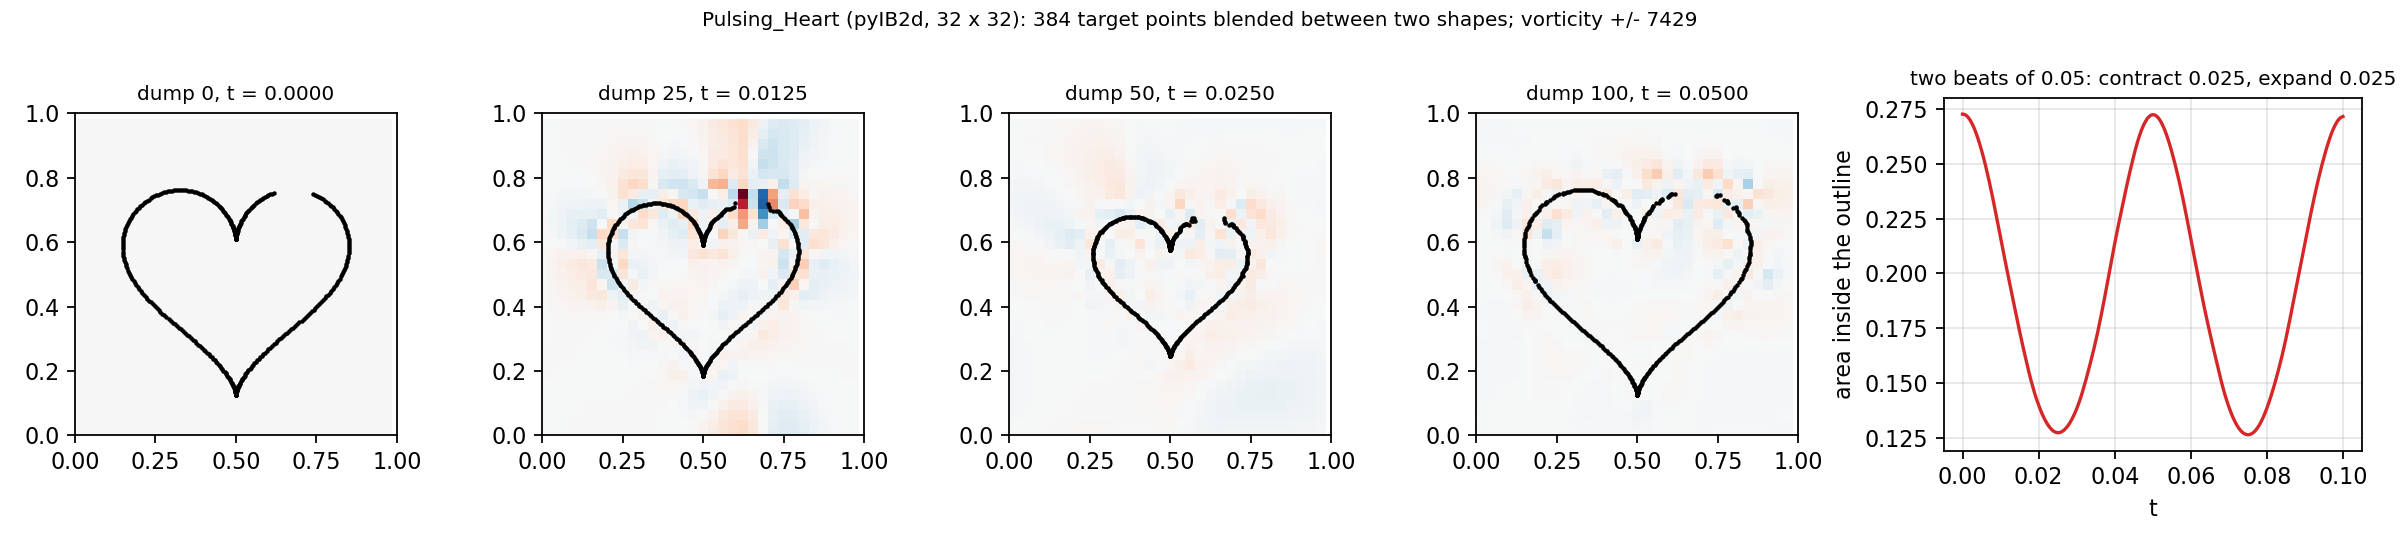
\includegraphics[width=\textwidth]{ch4c-pulsing-heart.png}
\footnotesize
\begin{itemize}
  \item 10\,000 steps in 24 s on a laptop; 201 dumps. The area inside the heart's outline (right) goes from 0.27 to 0.13 at the end of each contraction and back: the targets are followed exactly, beat after beat, because the motion is a function of time.
  \item The fluid is pushed out through the opening at the top during the contraction and drawn in during the expansion; at $32^2$ the vorticity at the opening's tips reaches $7 \cdot 10^3$ (the colour scale), the kind of number that says ``refine'' (chapter 4d). The example's $512 \times 512$ folder is a different model (6829 points, springs as well, its own update function), not a refinement of this one.
  \item The whole example is the data file, the blend and forty lines: the recipe of slide \ref{fr:phases} for any motion traced from images.
\end{itemize}
\end{frame}

% ---------------------------------------------------------------- your own example
\begin{frame}{Your own example: from a sketch to a folder}
\label{fr:own}
\small
\begin{enumerate}
  \item \al{Sketch the domain}: the box $[0, L_x] \times [0, L_y]$ with the origin at the corner (chapter 4a), the structure inside it with room for the flow it makes, the periodic edges in mind (a wall you want needs target points).
  \item \al{Choose the grid}: $N_x$, $N_y$ even, $\Delta x = \Delta y$ (so $L_x/N_x = L_y/N_y$: the sawtooth's $1024 \times 256$ for $12 \times 3$); start coarse ($32$--$64$ per unit length) and refine later (chapter 4d).
  \item \al{Place the points} at $\Delta s \approx \Delta x/2$ along the structure, by arc length, in an order you can describe (``points 0--827 are the top row''); print the counts the update function will need.
  \item \al{Decide the physics} per point: springs between neighbours (stretch), beams over triples (bend), target points where it is held or driven, masses where inertia matters; write the files with full precision and the right index base (0 in Python, 1 in MATLAB).
  \item \al{Write \code{input2d}} from a working example: the grid, $\mu$, $\rho$, $\Delta t$ and $T$, the flags that match the files you wrote, \code{string\_name}, \code{print\_dump}.
  \item \al{If it moves}, write the \code{update\_*} function in the second style (slide \ref{fr:styles}), with the counts read from the files.
  \item \al{Run short first}: $T$ of a few dumps, look at dump 0000 and 0001 (chapter 4b), then the console's ``FIBER MODEL INCLUDES'', then the full run.
\end{enumerate}
\end{frame}

\begin{frame}[fragile]{The course's template: two beams driven by target points}
\label{fr:twobeams}
\begin{columns}[T]
\column{0.5\textwidth}
\begin{lstlisting}[style=m]
Lx = 1;  Ly = 2;  N = 512;           % the longest side has N cells
dx = Ly/N;  ds = Ly/(2*N);           % ds should be 1/2 of dx
Lb = Lx/2;  npts_beam = ceil(Lb/ds); % 256 points per beam
mesh_name = 'two_beams_';
for s = 0:npts_beam-1                % the bottom beam, then the top one
   fprintf(vertex_fid, '%1.16e %1.16e\n', Lx/4+s*ds, Ly/2-Ly/8);
end
disp(['The vertex ids for the bottom beam go from 1 to ' num2str(npts_beam)]);
\end{lstlisting}
\small \code{generate\_meash.m} (sic), abridged.
\column{0.48\textwidth}
\begin{lstlisting}[style=m]
amp = 1/8;  freq = 1;  stop_time = 6;
first_bottom = 1;  last_bottom = 64;  first_top = 257;  last_top = 320;
yPTS = read_In_yPT_Positions('two_beams_512.vertex');
while current_time < stop_time
    for i = first_bottom:last_bottom
      targets(i,3) = yPTS(i) - amp*sin( 2*pi*freq*current_time );
    end
    for i = first_top:last_top
      targets(i,3) = yPTS(i) + amp*sin( 2*pi*freq*current_time );
    end
end
\end{lstlisting}
\small \code{update\_Target\_Point\_Positions.m}, abridged.
\end{columns}
\end{frame}

\begin{frame}{The template: what it does, and three things to fix}
\label{fr:twobeams2}
\small
\code{4-ib2d-MakeYourOwnExample} (the UA course, 2022): two horizontal beams of 256 points each in a $1 \times 2$ box, with springs, beams and target points (files \code{two\_beams\_512.*}), the beams' first quarters driven towards each other as a sine: a two-flap pump, with \code{read\_Vertex\_Points\_and\_Plot\_Them.m} to check it. It shows the recipe of the previous slide, and three things to fix before it runs:
\begin{itemize}
  \item \al{\code{while} must be \code{if}}: as written, the loop never ends when \code{current\_time < stop\_time} (nothing inside it changes the time): the run hangs in the first step.
  \item \al{Rows are not indices}: the generator writes target points for the first quarter of each beam only, so the \code{.target} file has 128 rows (rows 1--64 are points 1--64, rows 65--128 are points 257--320), but the function writes \code{targets(257:320, 3)}. MATLAB grows the table to 320 rows with zero indices, and the force routine then indexes \code{xLag(0)}: an error at the first step. Select rows 65--128, or the rows whose first column is between 257 and 320 (slide \ref{fr:table}).
  \item The counts are typed in (\code{64}, \code{257}, \code{320}) for one resolution; the \code{disp} lines of the generator are there to set them.
\end{itemize}
Fixed, it is the simplest pump you can write: exercise \ref{fr:exercises}.
\sourcecredit{The generator is called \code{generate\_meash.m} in the folder; the files are in IB2d's MATLAB numbering.}
\end{frame}

\begin{frame}{Checks before and after the first run}
\label{fr:checks}
\small
\begin{itemize}
  \item \al{The geometry}: the checker of chapters 4a and 6 (\code{test\_IB2d\_IBAMR\_Geometry}, \code{test\_ib\_geometry.py}) with the right index base; a plot from your generator; $\Delta s/\Delta x$ printed.
  \item \al{The files and flags agree}: every file your generator wrote has its flag at 1 and the right \code{string\_name}; every flag at 1 has its file (a missing file stops the run; a missing flag silently ignores the file: chapter 4a).
  \item \al{The update function is found and used}: the console's ``dynamically updating target point properties'' line; dump 0001 differs from dump 0000 where it should.
  \item \al{The counts}: print them from the function once (\code{N\_top}, the rows selected) and compare with the generator's output.
  \item \al{The motion}: plot the targets' path from the function alone, without the fluid (the swimmer's \code{test\_Script.m} does this; a five-line script that calls your function for a few times does the same), before spending the run.
  \item \al{Stability}: the first dumps at the chosen $\Delta t$; if the band or wall explodes, halve $\Delta t$ or soften the stiffness (slide \ref{fr:sawrun}; chapter 4d).
  \item \al{Resolution}: the same run at twice the grid, once, before any number from it is reported (chapter 4d).
\end{itemize}
\end{frame}

% ---------------------------------------------------------------- exercises, summary
\begin{frame}{Exercises}
\label{fr:exercises}
\small
\begin{enumerate}
  \item The course's homework: modify the rubber band so that it is 50\,\% smaller and deformed differently, with your own generator (Lectures 3 and 9); then drive it along a circle with an update function written in the second style (position as a function of time), and compare the band's centre with the prescribed path.
  \item On the full grid (MATLAB, or Python on a cluster), move the sawtooth's bottom row in antiphase (Lecture 3's line) and compare the flow rate through the middle with the one-row pump; then set the top row's amplitude so that its tips reach the bottom row's ($a = 2G$) and see what the occlusion does.
  \item Port the two-beam template to Python with the three fixes of slide \ref{fr:twobeams2}: a 256-point beam each, the first quarter of each driven; run it at $128 \times 256$ and plot the flow rate between the beams.
\end{enumerate}
\end{frame}

\begin{frame}{Exercises (2)}
\label{fr:exercises2}
\small
\begin{enumerate}
  \setcounter{enumi}{3}
  \item Take the moving band and halve $\Delta t$: compare the band's centre at $t = 0.025$ between the two runs for the increment style, then rewrite the function in the second style and compare again.
  \item Draw two phases of a shape of your own (a bell, a fin, a chamber), write them as the pulsing heart's four-column file, and run it with the same function; then change the blend to $\frac12(1 - \cos 2\pi t/P)$ and compare the vorticity at the opening.
  \item Design an example of your own from the project ideas of Lecture 2 (a barb moving towards a circle, a heart tube that pumps, a leaf that vibrates in a flow) following slide \ref{fr:own}; hand in the sketch, the generator, the function and the first two dumps.
\end{enumerate}
Lecture 11's homework 4, option 1: run an example related to your project instead. Appendix C collects the homework bank.
\end{frame}

\begin{frame}{Summary}
\label{fr:summary}
\footnotesize
\begin{itemize}
  \item A boundary moves in IB2d because something it is tied to changes in time: a target position, a resting length, a rest curvature, an activation. Each has a flag in \code{input2d} and a function in the example folder that the driver calls every step with the time and the current table, and whose returned table replaces it.
  \item The moving band increments the targets every step; the sawtooth sets them from the original positions as a function of time. Use the second style: no drift, the same motion at every $\Delta t$.
  \item The sawtooth's hard-coded \code{N\_top} and the two-beam template's \code{while} and row numbers are the classic mistakes of this kind of file: counts typed in for one resolution, a loop that was meant to be a condition, rows of the table confused with indices of the points. Read the counts from the files; test the function without the fluid.
  \item Coarsening a grid changes what a tethered wall can take: the sawtooth pump, built for $1024 \times 256$, failed on every laptop grid tried (stiff tethers blow up, soft ones let points stray two cells from their targets), while the pulsing heart at $32^2$ runs in half a minute; chapter 4d makes that a measurement.
  \item A new example is a sketch, a grid, points at $\Delta x/2$ in a known order, files with the right index base, an \code{input2d} copied from a working example, a short first run and a look at the first dumps.
  \item Next: chapter 4d, the stability and convergence lab.
\end{itemize}
\end{frame}

\begin{frame}{References and credits}
\label{fr:refs}
\scriptsize
\begin{itemize}
  \item The IB2d repository, \url{https://github.com/nickabattista/IB2d}: \code{matIB2d/Examples/Example\_Moving\_Rubberband} (\code{Rubberband.m}, \code{update\_Target\_Point\_Positions.m}), \code{Example\_Sawtooth} (\code{give\_Me\_Sawtooth\_Geometry.m}, \code{update\_Target\_Point\_Positions.m}, \code{input2d}, \code{Sawtooth\_Data\_Analysis.m}), \code{Example\_Pulsing\_Heart/32x32} (\code{All\_Positions.txt}, \code{update\_Target\_Point\_Positions.m}), \code{Examples\_First\_Year\_Seminar/Swimmer}; \code{pyIB2d/Examples/Tracers\_In\_Impedance\_Pump/update\_Springs.py}; the drivers' calls to the update functions (\code{IBM\_Driver.m} lines 805--821, \code{IBM\_Driver.py} lines 697--721). Code as of the 2024-03-06 clone.
  \item The Python ports and runs (October 2026): \code{examples/IB2d/Moving\_Rubberband}, \code{Sawtooth} and \code{Pulsing\_Heart} in this repository (the sawtooth variants tried: \code{wsl/final/ch4c\_saw*.sh}); \code{wsl/final/ch4c\_*.sh}; figures by \code{tools/ch4c\_figures.py} with \code{examples/analysis/read\_vtk\_legacy.py}.
  \item Sources merged (slide \ref{fr:sources}): ``Changing target positions'' (Lecture 3, UA 2022), Lectures 11 and 12 (2021--23), the 2024 practical (slide 29), ``IB2d and IBAMR associated files'' (Lecture 2, 2022), the UA ``4-ib2d-MakeYourOwnExample'' folder, ``Your own rubber band'' (the IBAMR Lecture 3 and Lecture 9 homework). Quotations are from those decks.
\end{itemize}
\end{frame}

\end{document}
